\documentclass[11pt]{article}
\usepackage[letterpaper,margin=1in]{geometry}
\usepackage[T1]{fontenc}
\usepackage{mathptmx}
\usepackage{courier}
\usepackage{amsmath,amssymb}
\usepackage{graphicx}
\usepackage{booktabs}
\usepackage{tabularx}
\usepackage[font=small,labelfont=bf]{caption}
\usepackage[numbers,sort&compress]{natbib}
\usepackage{xcolor}
\usepackage{listings}
\usepackage{microtype}
\usepackage{authblk}
\usepackage{tikz}
\usetikzlibrary{arrows.meta,positioning,fit}
\usepackage[colorlinks=true,linkcolor=blue!50!black,citecolor=blue!50!black,urlcolor=blue!50!black]{hyperref}
\renewcommand{\baselinestretch}{1.1}
\emergencystretch=2em
\renewcommand{\topfraction}{0.9}\renewcommand{\bottomfraction}{0.6}\renewcommand{\textfraction}{0.08}
\renewcommand{\floatpagefraction}{0.75}\setcounter{topnumber}{3}\setcounter{totalnumber}{5}
\newcommand{\chitwo}{\chi^{(2)}}
\newcommand{\um}{\,\mu\mathrm{m}}
\newcommand{\code}[1]{\texttt{#1}}
\lstset{basicstyle=\ttfamily\footnotesize,columns=fullflexible,frame=single,rulecolor=\color{black!25},backgroundcolor=\color{black!3},xleftmargin=4pt,xrightmargin=4pt,upquote=true,language=Python,keywordstyle=\bfseries,commentstyle=\itshape\color{black!60}}

\title{qwkit: an open, tested Python toolkit for quantum-well intersubband optics, from self-consistent states to saturated waveguide conversion}
\author{Gracen Ownby}
\affil{University of Oklahoma, Norman, Oklahoma, USA}
\date{\small 14 October 2026}

\begin{document}
\maketitle

\begin{abstract}
qwkit is a small, open-source Python package (MIT license) that computes the optical response of doped semiconductor quantum wells to infrared light, from the electron states of a layered structure to the harmonic power generated in a waveguide. Its core chains six calculations that are usually done with separate in-house codes: self-consistent Schr\"odinger--Poisson states with band nonparabolicity and depolarization; the resonant second-order susceptibility $\chitwo$ for arbitrary subband populations; LO-phonon intersubband scattering rates; multilevel saturation; planar waveguide modes and electrode fields; and coupled-mode propagation with pump depletion and quasi-phase matching. Five further modules add exact parameter sensitivities of the self-consistent model by implicit differentiation; the collective (time-dependent Hartree, random-phase) linear and second-order response, with and without in-plane dispersion; the two-dimensional electron gas at a single polar heterointerface; and intersubband thermal emitters at elevated temperature. Each module is checked by automated tests against analytic limits, exact symmetries, conservation laws or a published value (58 tests). The package has been used for a complete design study of electrically reversible quasi-phase matching in symmetric triple quantum wells, whose every number and figure it regenerates, and for six companion studies. The whole chain, from layer list to conversion efficiency, runs in under ten seconds on one processor core, most of it in the waveguide mode solver.
\end{abstract}

\section{Summary}
Electrons confined in quantum wells (QWs) a few nanometres thick occupy discrete subbands, and transitions between them, intersubband (ISB) transitions, can be placed anywhere in the mid- and far-infrared by choosing layer thicknesses. Coupling two or three such transitions resonantly with a pump and its harmonic produces second-order nonlinearities $\chitwo$ that exceed those of bulk crystals by orders of magnitude \cite{Fejer1989,Rosencher1991,Vurgaftman2021}. These nonlinearities drive difference-frequency terahertz sources in quantum cascade lasers \cite{Belkin2007}, giant and electrically tunable nonlinear metasurfaces \cite{Lee2014,Yu2022}, and waveguide frequency converters \cite{Chesi2023}. Predicting what a given structure will do requires a chain of calculations: subband states in the structure's own electrostatic potential, collective (depolarization) shifts of the transitions, the susceptibility for the actual subband populations, how fast excited electrons relax, how the populations saturate under strong pumping, how the light is confined in a waveguide, and how the harmonic builds up along it.

qwkit implements this chain, and the extensions described below, in about 2500 lines of documented Python that depend only on NumPy and SciPy. A user describes a structure as a list of layers, applies a field and a doping level, and obtains energies, dipoles, $\chitwo$, absorption, scattering rates, saturation curves, waveguide modes and conversion efficiencies, and, with the extension modules, parameter sensitivities, collective spectra and thermal emission spectra, all through plain functions and dictionaries that can be inspected at every stage.

\section{Statement of need}
Design studies of ISB nonlinear devices are often carried out with in-house codes, and the steps of the chain are frequently reported separately: a band-structure calculation in one paper, a susceptibility estimate in another, a propagation model with a single assumed relaxation time in a third. This makes results hard to reproduce and hides model choices that change conclusions. Three examples arose while developing the package. A susceptibility formula written with diagonal dipole elements measured from an arbitrary origin produces a spurious $\chitwo$ in a perfectly symmetric structure. Replacing a common 1~ps relaxation time with level-resolved LO-phonon rates lowers absolute conversion efficiencies at watt-level pumping by factors of 1.3--1.8 at 1.26~W and 1.2--4.2 at 10~W, depending on the phase-matching scheme. And an ``idealized'' benchmark that keeps the on-state absorption in switched-off segments understates a competing, Stark-modulated quasi-phase-matching (QPM) scheme by 1.6--25 times at 1.26--20~W \cite{Ownby2026N1}. An open, tested implementation of the whole chain lets such choices be stated, varied and checked.

The intended users are researchers and students who design or interpret ISB absorbers, emitters, modulators and nonlinear converters; those who want a transparent reference implementation of standard ISB formulas \cite{Vurgaftman2021}; and those who need a fast, scriptable forward model, with exact derivatives, for optimization or uncertainty studies.

\section{State of the field}
Table~\ref{tab:field} compares qwkit with widely used open and commercial codes for semiconductor heterostructures, as their authors describe them. General-purpose packages solve the Schr\"odinger--Poisson problem in one to three dimensions with multiband $\mathbf{k}\cdot\mathbf{p}$ models \cite{Birner2007,Hebal2021,Beugeling2025}; quantum-cascade-laser tools design laser active regions \cite{ErwinJr2}; and solar-cell libraries couple QW absorption to device transport \cite{AlonsoAlvarez2018,Gaury2019}. As far as their publications and documentation describe, none of the open codes combines depolarization-shifted transitions, a population-resolved resonant $\chitwo$, LO-phonon relaxation, multilevel saturation, waveguide modes and saturable coupled-mode propagation in one tested chain. qwkit is deliberately narrower than the general-purpose codes: it is a one-dimensional, single-conduction-band code for the ISB optics of electron-doped structures (with a two-band Kane cross-check of its dipoles), and it does not replace multiband $\mathbf{k}\cdot\mathbf{p}$ or transport solvers.

\begin{table}[t]
\centering\small
\caption{Heterostructure codes as described by their authors, and the scope of qwkit.}\label{tab:field}
\begin{tabularx}{\textwidth}{@{}lXl@{}}
\toprule
Code & Scope (from its publication or documentation) & Availability \\ \midrule
nextnano \cite{Birner2007} & General-purpose 1D--3D Schr\"odinger--Poisson and $\mathbf{k}\cdot\mathbf{p}$ device simulation, including intersubband scattering times and absorption \cite{nextnanoBench} & Proprietary \\
Aestimo 1D \cite{Hebal2021} & 1D self-consistent Schr\"odinger--Poisson, single-band or multiband $\mathbf{k}\cdot\mathbf{p}$ & Open (GPL v3) \\
kdotpy \cite{Beugeling2025} & Kane-model $\mathbf{k}\cdot\mathbf{p}$ on a lattice for band structures & Open \\
ErwinJr2 \cite{ErwinJr2} & Quantum cascade laser design: 1D eigenstates, LO-phonon scattering, optical gain and threshold current, transfer-matrix waveguide optics and confinement factor, with a GUI & Open \\
Solcore \cite{AlonsoAlvarez2018} & Multi-scale solar-cell modelling, including QW band structure and absorption & Open \\
Sesame \cite{Gaury2019} & 2D drift-diffusion solar-cell modelling & Open \\
\textbf{qwkit} & 1D one-band ISB optics: nonparabolic self-consistent states, depolarization, $\chitwo$, LO-phonon rates, saturation, waveguide modes, electrode fields, coupled-mode SHG with QPM; implicit-differentiation sensitivities, collective (RPA) $\chi^{(1)}$ and $\chitwo$, single-heterointerface 2DEG, ISB thermal emitters & Open (MIT) \\ \bottomrule
\end{tabularx}
\end{table}

\section{Software design}
\subsection{Architecture}
The package has eleven modules (Fig.~\ref{fig:arch}): six that form the chain from layer list to conversion efficiency, and five extensions that use the same states and conventions. Each is a set of plain functions operating on NumPy arrays and dictionaries, so any intermediate quantity can be inspected, modified or replaced. The few classes hold precomputed data: \code{propagation.Medium} holds a saturable medium built from a ``state set'' dictionary (energies, dipoles, shifted transition energies, populations, density), which \code{sp.state\_set} produces from a self-consistent solution; \code{tdh.TDH} and \code{krpa.KRPA} hold the Hartree kernel and unperturbed density matrix of a response calculation; and \code{sens.Model} holds the parameter vector of the differentiable model.

\begin{figure}[t]
\centering
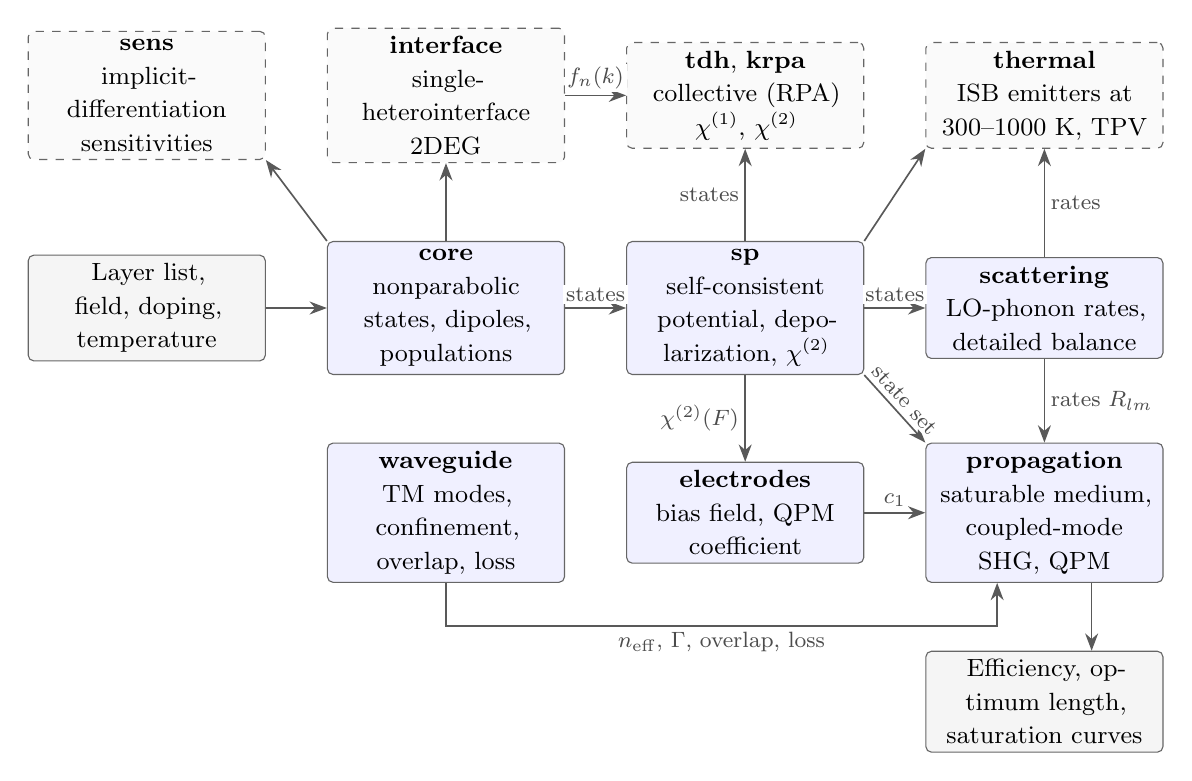
\begin{tikzpicture}[font=\small,
  box/.style={draw=black!60, rounded corners=2pt, fill=#1, align=center, minimum height=12mm, text width=28mm, inner sep=3pt},
  box/.default={blue!6},
  ext/.style={draw=black!60, dashed, rounded corners=2pt, fill=black!2, align=center, minimum height=12mm, text width=28mm, inner sep=3pt},
  arr/.style={-{Stealth[length=2.2mm]}, black!65, line width=0.6pt},
  lab/.style={font=\footnotesize, black!70, fill=white, inner sep=1pt}]
\node[box=black!4] (in) at (0,0) {Layer list, field, doping, temperature};
\node[box] (core) at (3.8,0) {\textbf{core}\\ nonparabolic states, dipoles, populations};
\node[box] (sp) at (7.6,0) {\textbf{sp}\\ self-consistent potential, depolarization, $\chitwo$};
\node[box] (sc) at (11.4,0) {\textbf{scattering}\\ LO-phonon rates, detailed balance};
\node[box] (wg) at (3.8,-2.6) {\textbf{waveguide}\\ TM modes, confinement, overlap, loss};
\node[box] (el) at (7.6,-2.6) {\textbf{electrodes}\\ bias field, QPM coefficient};
\node[box] (prop) at (11.4,-2.6) {\textbf{propagation}\\ saturable medium, coupled-mode SHG, QPM};
\node[box=black!4] (out) at (11.4,-5.0) {Efficiency, optimum length, saturation curves};
\draw[arr] (in) -- (core);
\draw[arr] (core) -- node[lab, above=1pt]{states} (sp);
\draw[arr] (sp) -- node[lab, above=1pt]{states} (sc);
\draw[arr] (sc) -- node[lab, right=1pt]{rates $R_{lm}$} (prop);
\draw[arr] (sp) -- node[lab, left=1pt]{$\chitwo(F)$} (el);
\draw[arr] (sp.south east) -- node[lab, sloped, above=1pt]{state set} (prop.north west);
\draw[arr] (el) -- node[lab, above=1pt]{$c_1$} (prop);
\draw[arr] (wg.south) -- ++(0,-0.55) -| node[lab, pos=0.25, below=1pt]{$n_\mathrm{eff}$, $\Gamma$, overlap, loss} ([xshift=-6mm]prop.south);
\draw[arr] ([xshift=6mm]prop.south) -- ([xshift=6mm]out.north);
\node[ext] (sens) at (0,2.7) {\textbf{sens}\\ implicit-differentiation sensitivities};
\node[ext] (intf) at (3.8,2.7) {\textbf{interface}\\ single-heterointerface 2DEG};
\node[ext] (tdh) at (7.6,2.7) {\textbf{tdh}, \textbf{krpa}\\ collective (RPA) $\chi^{(1)}$, $\chitwo$};
\node[ext] (th) at (11.4,2.7) {\textbf{thermal}\\ ISB emitters at 300--1000~K, TPV};
\draw[arr] (core.north west) -- (sens.south east);
\draw[arr] (core) -- (intf);
\draw[arr] (intf) -- node[lab, above=1pt]{$f_n(k)$} (tdh);
\draw[arr] (sp) -- node[lab, left=1pt]{states} (tdh);
\draw[arr] (sp.north east) -- (th.south west);
\draw[arr] (sc) -- node[lab, right=1pt]{rates} (th);
\end{tikzpicture}
\caption{Module structure and data flow. Solid boxes form the chain from layer list to conversion efficiency; dashed boxes are the extension modules. Each arrow is a plain array or dictionary passed from one module to the next; $c_1$ is the QPM Fourier coefficient and $R_{lm}$ the LO-phonon rate matrix.}
\label{fig:arch}
\end{figure}

\subsection{Physics and numerical choices}
\paragraph{States.} The Schr\"odinger equation with the BenDaniel--Duke operator \cite{BenDaniel1966} and Kane nonparabolicity $m^*(z,E)=m_\mathrm{edge}(z)[1+(E-V(z))/E_g(z)]$ \cite{Nelson1987}, with InGaAs/InAlAs band parameters from Ref.~\cite{Vurgaftman2001}, is discretized on a cell-centred grid and solved with a tridiagonal eigensolver. Two choices make symmetric structures exactly symmetric numerically, which matters because a field-induced $\chitwo$ is a small difference of large terms. First, no grid node sits on an interface, so mirror-symmetric stacks give mirror-symmetric matrices. Second, each nonparabolic state is found by \emph{index tracking}: the $k$-th state satisfies $E=$ the $k$-th eigenvalue of $H(E)$, which preserves node counting, whereas matching states by nearest energy can swap or duplicate them. States from different energy-dependent Hamiltonians are not exactly orthogonal; they are L\"owdin-orthonormalized \cite{Lowdin1950}, which preserves parity and changes them minimally, together with at least ten box states above the highest localized one (solved at the converged potential if needed), and only then truncated to the states a calculation keeps (\code{core.lowdin\_localized}, used by \code{sp.prepare}; \code{sens} and \code{thermal} orthonormalize all their model states before selecting). The buffer matters when few states are localized: the topmost localized state cannot be orthogonalized against states left out of the set. As an exact alternative, \code{core.kane\_dipoles} forms dipoles from the two-component states of the two-band Kane model behind the energy-dependent mass (conduction envelope plus valence component), which are orthogonal without this step. The simulation box is closed by hard walls ($\psi=0$ one grid step beyond each end), and \code{core.localized} separates the states of the active region from the continuum-like states of the padded box. Only the tracked eigenpair is computed at each iteration, and the energy-dependent mass is updated by a secant iteration.

\paragraph{Electrostatics.} For a voltage-biased periodic stack, the period-averaged field equals the applied field and the Hartree field has zero mean over a period. Poisson's equation is solved with position-dependent permittivity using centred cumulative integrals (a forward sum breaks the symmetry at second order), and iterated with linear mixing and warm starts. Depolarization shifts follow Ando \emph{et al.} \cite{Ando1982}, transition by transition, with a user-set average permittivity.

\paragraph{Susceptibility.} The resonant SHG susceptibility for arbitrary populations $\rho_l$ is evaluated as the full density-matrix sum \cite{Boyd2008,Rosencher1991}
\begin{equation}
\chitwo(2\omega)=\frac{Ne^3}{\varepsilon_0}\sum_{l,m,n}\frac{z_{lm}z_{mn}z_{nl}}{\tilde E_{nl}-2\hslash\omega-i\Gamma}\left[\frac{\rho_l-\rho_m}{\tilde E_{ml}-\hslash\omega-i\Gamma}-\frac{\rho_m-\rho_n}{\tilde E_{nm}-\hslash\omega-i\Gamma}\right],
\end{equation}
where $N$ is the period-averaged electron density, $\rho_l$ the fractional population of subband $l$ ($\sum_l\rho_l=1$), $z_{lm}$ the dipole matrix elements, $\tilde E_{ml}=-\tilde E_{lm}$ the depolarization-shifted transition energies and $\Gamma$ the half-width at half-maximum. The sum is invariant under a shift of the coordinate origin and contains the permanent-dipole terms automatically. Because $\chitwo$ and the ISB absorption are linear in $\rho$, \code{Medium} precomputes them as coefficient vectors, so saturation can be re-evaluated at every propagation step at negligible cost.

\paragraph{Relaxation and saturation.} Intersubband LO-phonon rates use the Fr\"ohlich interaction with bulk phonons for electrons at the subband minimum \cite{Ferreira1989}; the form factor $\iint\psi_l\psi_m(z)\psi_l\psi_m(z')e^{-Q|z-z'|}dz\,dz'$ is evaluated in $O(N)$ operations with running exponential sums, and upward rates follow from detailed balance. For the extension modules, \code{scattering} also provides rates for several polar-phonon modes with per-mode Fr\"ohlich weights and Thomas--Fermi screening, a static random-phase screening factor with Coulomb form factors, and $k$-resolved rates with an angular integral, a nonparabolic final density of states and Pauli blocking. Steady-state populations under pump and harmonic intensities solve a linear rate system in which either a single relaxation time or the level-resolved rate matrix returns the populations to equilibrium.

\paragraph{Waveguide, electrodes and propagation.} TM modes of planar multilayer guides with complex permittivities (InP dispersion \cite{Pettit1965}, Drude free carriers, gold \cite{Ordal1985}) are found by finite differences for $H_y$. Fields under alternating-polarity electrodes come from a Fourier-series solution of Laplace's equation for a uniform permittivity, and the QPM coefficient is the first Fourier component of $\chitwo(F(x))$ \cite{Fejer1992}. Mode amplitudes are propagated with fourth-order Runge--Kutta, including pump depletion, saturable losses and either a periodic QPM pattern (\code{propagate}) or a sequence of different media, each one coherence length long (\code{propagate\_segments}), which describes Stark on/off QPM realistically.

\paragraph{Sensitivities.} \code{sens} gives exact first-order derivatives of the one-period self-consistent model with respect to layer thicknesses, field, doping, band offset, masses, nonparabolicity gaps and permittivities, by implicit differentiation of the converged Hartree fixed point. Interfaces are smoothed by an error function one grid cell wide, so every material profile is differentiable in the interface positions. State tangents follow from first-order perturbation theory of the nonparabolic eigenproblems at fixed total density. They are computed matrix-free: reduced resolvents are applied by shifted tridiagonal LU solves with projection and iterative refinement, and the Hartree feedback $(I-K)\,\delta V_H=b$ is solved by GMRES (typically five iterations), so neither a full eigendecomposition nor an explicit density-response matrix is formed (the dense route remains as an option and agrees to $10^{-8}$). The closed-form post-processing (L\"owdin step over all model states, about ten more than are kept, then dipoles, depolarization shifts, $\chitwo$, absorption and a waveguide figure of merit) is differentiated along each tangent by Richardson-extrapolated central differences, on the most localized states rather than the lowest ones, so a delocalized box state is never selected.

\paragraph{Collective response.} \code{tdh} solves the density-matrix equations of one period with the time-dependent Hartree (random-phase) potential of the induced charge, the drive being referenced to the displacement field. It returns $\chi^{(1)}$ and $\chitwo$ by frequency-domain perturbation theory and integrates the full nonlinear response in real time (fourth-order Runge--Kutta). For two levels its kernel reproduces Ando's depolarization shift, and without the kernel the density-matrix $\chitwo$ above is recovered. \code{krpa} generalizes it from subband populations to Fermi occupations on in-plane wavevector shells with nonparabolic dispersions and a frequency-dependent (polar-phonon) background permittivity, for linear and second-order response; only pairs with an occupation difference carry first-order coherences, and an adiabatic local exchange--correlation kernel is optional. With a single shell it reduces exactly to \code{tdh}.

\paragraph{Heterointerface and thermal emitters.} \code{interface} computes the two-dimensional electron gas at a single polar heterointerface self-consistently: Kane-nonparabolic subbands with an in-plane dispersion and density of states consistent with the same Hamiltonian, Fermi-level pinning by compensating acceptors over a depletion layer, a positive sheet at the interface and the cap surface or a fixed interface sheet (electric-double-layer gating), an optional fixed ionized-donor density in the cap (for example oxygen vacancies created by an electrolyte) with the remaining positive charge placed on the cap surface, at the interface or in the donors, and optional Hedin--Lundqvist exchange--correlation, with Anderson mixing. \code{thermal} supplies temperature-dependent material data (Varshni gaps, $\Gamma$--L separations, L-valley masses), intrinsic densities, the self-consistent period at temperature with continuum states and an L-valley reservoir, ISB absorption with thermal populations and $k$-resolved in-plane nonparabolicity, LO-phonon linewidths, an Urbach-tail interband background, coupled-mode emissivity, generation leakage and two-surface thermophotovoltaic (TPV) detailed balance.

\subsection{Design trade-offs}
The package favours transparency and verifiability over generality. A one-band model with Kane nonparabolicity describes conduction-band ISB transitions in narrow- and moderate-gap III--V wells well \cite{Nelson1987,Sirtori1994} and makes every matrix element inspectable; valence-subband and interband problems are out of scope until a multiband module exists (\code{thermal} includes interband absorption only as a bulk Urbach tail). Plain functions and dictionaries were chosen over an object hierarchy so that a study can stop after any step, swap in a different model, and keep its inputs and outputs as JSON. Units are fixed per module (\AA{} and eV in the state, interface and response solvers, pm/V for their $\chitwo$; SI for media in \code{propagation}, with waveguide inputs in $\mu$m and cm$^{-1}$; metres in \code{electrodes}) and are listed in the user guide. Steady-state rate equations assume pulses much longer than the picosecond relaxation times, and the waveguide is planar; both are stated limitations rather than hidden ones.

\begin{lstlisting}[float=t,caption={From layers to conversion efficiency (abridged from \code{docs/examples.py}).},captionpos=b,label=lst:ex]
from qwkit import sp, scattering, propagation
HW = 1.23984 / 10                                    # 10 um pump photon energy (eV)
TW = [(58, "well"), (14, "barrier"), (34, "well"), (14, "barrier"), (58, "well")]
o = sp.chi2_sc(TW, 55.0, HW, ns_cm2=5e11)            # o["chi"]: chi(2) in pm/V
E, psi, Z, rho = sp.prepare(o["r"])
R = scattering.rate_matrix(o["r"]["z"], psi, E)      # LO-phonon rates (1/s)
med = propagation.Medium(sp.state_set(o), HW, R=R)    # saturable medium
wg = dict(n1=3.231, n2=3.338, G1=0.395, G2=0.514, O_um=0.0531, abg1_cm=3.25,
          abg2_cm=0.16, t_stack_um=1.512, w_um=15.0, Lcoh_um=23.4, lam1_um=10.0)
# wg: from waveguide.tm_modes and shg_overlap; eta_e: QPM coefficient from electrodes
res = propagation.propagate(med, wg, 1.26, "sign", eta_e=0.92, L_max_um=500)
print(res["eta"], res["L_opt_um"])                   # peak efficiency, length
\end{lstlisting}

\section{Validation}
Each module is checked against independent references (Table~\ref{tab:val}); the 58 tests run in about 40~s on one core. Fig.~\ref{fig:val} shows four of them. Subband energies of a finite InGaAs/InAlAs well agree with the analytic BenDaniel--Duke solution to 0.04~meV on the default 0.5~\AA{} grid, with second-order convergence (Fig.~\ref{fig:val}a). In a self-consistent mirror-symmetric triple well, $|\chitwo(F)+\chitwo(-F)|$ stays below $4\times10^{-11}|\chitwo|$ at every field (Fig.~\ref{fig:val}b), more than four orders of magnitude below the test tolerance. With the parameters of a published reproduction of Ferreira and Bastard's calculation \cite{Ferreira1989,nextnanoBench} ($m^*=0.07$, conduction-band offset 0.2138~eV, $\varepsilon_s=12.5$, $\hslash\omega_\mathrm{LO}=36$~meV, $T=0$; that source does not state $\varepsilon_\infty$, for which we take 10.89), the LO-phonon emission time of a 10~nm GaAs well is 0.73~ps, against the published 0.83~ps (Fig.~\ref{fig:val}c). The 13\% difference is of the size produced by plausible choices of $\varepsilon_\infty$ (a value of 11.07 reproduces 0.83~ps), so this test guards the magnitude of the rates rather than fixing their last digit. The coupled-mode solver reproduces the phase-mismatched $\mathrm{sinc}^2$ solution to $10^{-6}$ and the $(2/\pi)^2$ factor of sign-reversal QPM (Fig.~\ref{fig:val}d), and, with 256 steps per coherence length, conserves total power to $10^{-6}$ in a strongly depleted lossless case. The extension modules are checked in the same way: the sensitivities against central finite differences, including cells where the energy-dependent mass reaches its floor, and the matrix-free against the dense tangents; the collective response against the single-particle $\chitwo$, Ando's shift and its own real-time integration; \code{krpa} against \code{tdh}; and the interface and thermal modules against closed-form densities, Gauss's law, the Stefan--Boltzmann law and detailed-balance limits.

Corrections made after the first release change results slightly. The ends of the simulation box were zero-flux (Neumann) boundaries, although documented as hard walls; they are now Dirichlet ($\psi=0$ one step beyond each end). Bound states of padded structures are unchanged (by less than $10^{-4}$~meV for 100~\AA{} pads), while continuum-like box states shift and spurious states localized at the box edges disappear. The nonparabolic states are now L\"owdin-orthonormalized together with at least ten box states above the localized ones before the basis is truncated. Orthonormalizing an already truncated set gave its topmost states spurious dipoles (up to 3\% of the $1\to n$ oscillator strength in a capped basis of the heterointerface study), and so did orthonormalizing the localized states alone when only a few are localized: for the 64/10/29~\AA{} double well in a 200~\AA{} box, with three localized states, $z_{13}$ came out 8.77~\AA{} against 8.22~\AA{} from the two-band Kane states, and $|\chitwo|$ about 8\% too large. The two-band Kane states provide this independent check of the L\"owdin step: for six asymmetric double wells and the symmetric triple well at zero bias, the localized two-component states overlap by less than $10^{-4}$ (against 0.04--0.07 for the raw one-band states); with the buffered step the one-band dipoles agree with the Kane dipoles to within 0.7\% and do not depend on the box size, and computing the peak ground-state $\chitwo$ of the double wells with the Kane dipoles changes it by $-0.2$ to $-0.6\%$. The studies built on qwkit were re-run after these corrections.

\begin{figure}[t]
\centering
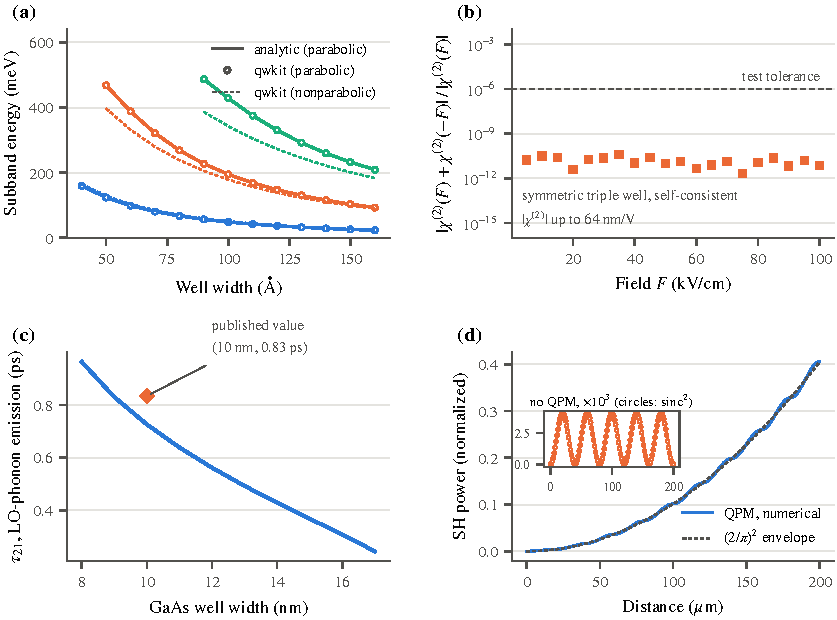
\includegraphics[width=0.86\textwidth]{figures/fig_validation.pdf}
\caption{Validation. (a) Subband energies of a finite InGaAs/InAlAs well (0.52~eV offset, masses 0.043/0.075) vs width: analytic BenDaniel--Duke solution (lines), qwkit with parabolic bands (circles) and with nonparabolicity (dashed). (b) Odd-symmetry residual of $\chitwo$ in a self-consistent symmetric 58/14/34/14/58~\AA{} triple well ($n_s=5\times10^{11}$~cm$^{-2}$), with the test tolerance. (c) LO-phonon emission time of a GaAs/Al$_{0.3}$Ga$_{0.7}$As well vs width with the parameters stated in the text, and the published value. (d) Second-harmonic power along a lossless guide ($L_\mathrm{coh}=20\um$), normalized to the perfectly phase-matched power at 200$\um$: sign-reversal QPM against its $(2/\pi)^2$ envelope, and the unmatched case (inset, enlarged) against the analytic $\mathrm{sinc}^2$ solution.}
\label{fig:val}
\end{figure}

\begin{table}[tp]
\centering\small
\caption{Automated validation tests in the version described here (58 tests, all pass). Quantities not yet covered by a dedicated test: free-carrier and metal losses in the waveguide, electrode fields with finite gaps, the WKB escape estimates, and the thermal emitter state and leakage.}\label{tab:val}
\begin{tabularx}{\textwidth}{@{}lX@{}}
\toprule
Quantity & Reference and criterion \\ \midrule
Subband energies & Infinite well (energies within 1\%, $z_{12}$ within 2\%); finite well with BenDaniel--Duke matching (0.1~meV, second-order convergence) \\
Populations & Two-dimensional Fermi--Dirac closed form ($10^{-12}$) \\
States with nonparabolicity & Exact parity and strictly ordered energies; mirror-image structures give identical $|z_{ij}|$ under an origin shift ($10^{-6}$); two-band Kane states orthogonal ($2\times10^{-3}$) with $z_{12}$ within 2\% of the L\"owdin value; buffered L\"owdin dipoles of a double well with three localized states vs Kane dipoles (1.2\%) and independent of the box size (1\%) \\
$\chitwo$ & Three-level textbook limit \cite{Vurgaftman2021} (5\%); translation invariance ($10^{-9}$); $\chitwo(0)=0$ and $\chitwo(-F)=-\chitwo(F)$ for fixed and self-consistent potentials ($10^{-6}$) \\
Electrostatics & Charged sheets vs analytic (1\%); continuity of $D$ across a dielectric interface and zero-mean field ($10^{-6}$); neutrality and convergence ($10^{-5}$~eV) \\
Depolarization & Infinite-well shift vs closed-form $S_{12}=5L/9\pi^2$ ($10^{-4}$); blue shift for a populated ground state; vanishes as $n_s\to0$ \\
LO-phonon rates & Form factor vs direct double sum ($10^{-9}$) and short-range limit (1\%); published GaAs benchmark (15\%); detailed balance ($10^{-6}$); multimode and $k$-resolved rates reduce to the single-mode band-edge rate ($10^{-12}$, $10^{-6}$); Pauli blocking and screening lower the rate \\
Saturation & Two-level limit (absorption halves at $I_\mathrm{sat}$); cross-section scaling with refractive index; level-resolved equilibrium stationary, populations conserved \\
Waveguide, electrodes & Symmetric slab TM$_0$ index ($2\times10^{-4}$); mode normalization and confinement ($10^{-9}$); parallel-plate field (1\%); QPM coefficients $2/\pi$ and $1/\pi$ ($10^{-3}$) \\
Propagation & Undepleted phase-matched limit ($10^{-3}$); phase-mismatched $\mathrm{sinc}^2$ limit ($10^{-6}$); power conservation ($10^{-6}$ at 256 steps per coherence length); segmented media reproduce sign reversal ($10^{-6}$) \\
Sensitivities & Implicit derivatives vs central finite differences: energies (relative $2\times10^{-4}$), states and occupations ($10^{-3}$), and seven observables for all parameter types ($2\times10^{-3}$), also with the mass floor active; matrix-free vs dense tangents ($10^{-8}$) \\
Collective response & Bare limit vs density-matrix $\chitwo$ (1\%); linear peak at the Ando energy (0.3~meV); real time vs second order ($10^{-3}$, $2\times10^{-3}$); \code{krpa} with one shell, or with inactive pairs, vs \code{tdh} ($10^{-9}$ for $\chi^{(1)}$, $10^{-8}$ for $\chitwo$); shell occupations vs subband densities ($2\times10^{-3}$); Fr\"ohlich weights sum to $1/\varepsilon_\infty-1/\varepsilon_s$ ($10^{-12}$) \\
Heterointerface & Subband densities vs Fermi--Dirac closed form ($2\times10^{-4}$) and degenerate nonparabolic limit ($10^{-3}$); neutrality ($10^{-6}$), flat potential beyond the depletion edge and Fermi-level pinning (5~meV); Hedin--Lundqvist potential ($10^{-9}$); inverse in-plane dispersion; cap donors leave the subband spacing unchanged (Gauss's law, 2~meV) and bend the cap band down; neutrality with the remaining positive charge in the donors or at the interface ($10^{6}$~cm$^{-2}$) \\
Thermal emitters & Varshni gaps of GaAs and InGaAs (2~meV) and GaAs intrinsic density; Planck flux vs Stefan--Boltzmann ($10^{-4}$); critical coupling gives unit emissivity ($10^{-3}$); TPV efficiency below Carnot, narrowband emitter more efficient and less powerful; temperature-independent ISB line strength in the parabolic limit (2\%) \\ \bottomrule
\end{tabularx}
\end{table}

\section{Research use and performance}
qwkit was built for, and used in, a complete design study of electrically reversible QPM in mirror-symmetric InGaAs/InAlAs triple quantum wells \cite{Ownby2026N1}. The study's scripts, distributed with the package, regenerate every number and figure of that manuscript from the layer list: self-consistent model ladders and error budgets, LO-phonon-resolved saturation, waveguide and electrode design, and propagation comparisons against bipolar-biased, Stark-modulated and growth-reversed benchmarks. Fig.~\ref{fig:ex} shows three stages of that workflow. The extension modules were developed for six companion studies whose scripts are also distributed: saturation limits of resonant ISB second-harmonic generation \cite{OwnbyNL02}, collective effects in the resonant $\chitwo$ (\code{tdh}) \cite{OwnbyNL05}, temperature limits of bias-switchable ISB thermal emitters (\code{thermal}) \cite{OwnbyTPV05}, ISB optics of the polar LaInO$_3$/BaSnO$_3$ electron gas (\code{interface}, \code{krpa}) \cite{OwnbyMAT01}, electrolyte gating of the same interface (\code{interface}) \cite{OwnbyMAT02}, and sensitivities, uncertainty quantification and growth-tolerant design (\code{sens}) \cite{OwnbyMS02}. Developing the study, and an independent review of the package, exposed and fixed several subtle errors that the tests now guard against: spurious $\chitwo$ in symmetric structures from grid asymmetry, state swapping and non-orthogonality; an asymmetric Hartree integral; a zero-mean condition imposed on the field rather than through the displacement, which broke continuity of $D$ at dielectric interfaces (changing $|\chitwo|$ by at most 0.1\%); and a Runge--Kutta stage that sampled the next domain's QPM sign at domain edges.

On one core of a 2.8~GHz Xeon, a self-consistent solution with seven states on a 0.5~\AA{} grid takes about 0.4~s, the LO-phonon rate matrix a few milliseconds, and a saturable, pump-depleted propagation over 500$\um$ (about 700 steps) about 0.15~s. The TM mode of the waveguide, a dense eigenproblem on a 0.02$\um$ grid, takes about 4~s per wavelength, and is needed once per waveguide design. The sensitivities of a self-consistent solution with respect to all 12--14 parameters of a double or triple well cost about a sixth to a fifth of its converged forward solve (0.18--0.34~s against 1.1--1.5~s). Parameter scans of thousands of designs are therefore practical on a workstation.

\begin{figure}[t]
\centering
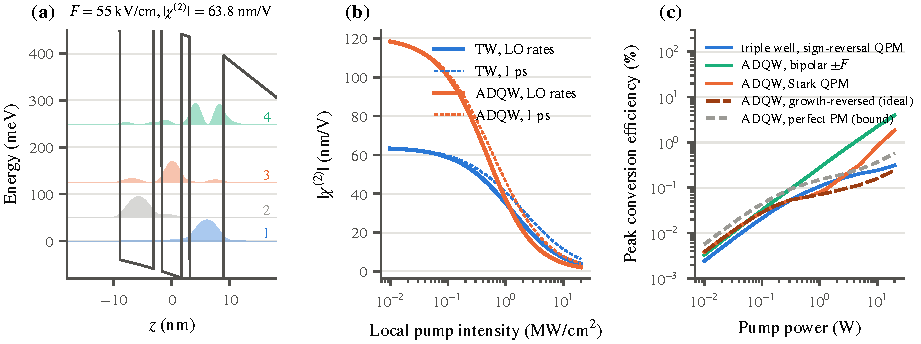
\includegraphics[width=\textwidth]{figures/fig_example.pdf}
\caption{An end-to-end example at $n_s=5\times10^{11}$~cm$^{-2}$ per period and a 10$\um$ pump. (a) Self-consistent conduction band and the densities of subbands 1--4 (bottom to top) of a 58/14/34/14/58~\AA{} InGaAs/InAlAs triple well at 55~kV/cm. (b) $|\chitwo|$ vs local pump intensity for the triple well (TW) and a 64/10/29~\AA{} asymmetric double quantum well (ADQW), with LO-phonon rates and with a single 1~ps time. (c) Peak conversion efficiency vs pump power in the waveguide of Ref.~\cite{Ownby2026N1} for the triple well with sign-reversal QPM at 55~kV/cm and four ADQW schemes (bipolar bias $\pm F$ and Stark QPM, each with optimized fields; ideal growth-defined reversal; perfect phase matching), from that study's distributed outputs.}
\label{fig:ex}
\end{figure}

\section{Limitations and development plan}
qwkit treats conduction-band ISB physics in one dimension with a single band; the two-band Kane states serve only as a cross-check of the dipoles. Three of the extensions planned at the first release are now included: thermal subband populations and linewidths for high-temperature ISB emitters (\code{thermal}), exact derivatives for gradient-based design under growth tolerances (\code{sens}), and a collective (multisubband-plasmon) response beyond first-order depolarization (\code{tdh}, \code{krpa}). The next planned extension is an interband and carrier-escape module (hole subbands, interband absorption, tunnelling and thermionic escape) for QW solar cells and thermophotovoltaic absorbers. The saturable propagation still uses first-order depolarization, Lorentzian lines and LO-phonon relaxation only. New alloys can be registered with \code{add\_material}; the padding material, the density-of-states mass, the depolarization permittivity and the LO-phonon parameters are function arguments, so other III--V systems need only parameter sets and validation; \code{interface} and \code{krpa} accept several polar-phonon modes and have been applied to a polar oxide, while nonpolar or strongly anisotropic materials need new scattering models.

\section{Availability}
The version described here is release 0.6.1; its changes since 0.5.0 are listed in \code{CHANGELOG.md}. It requires Python $\geq$3.10, NumPy and SciPy (Matplotlib for figures). It installs with \mbox{\code{pip install .}} and is released under the MIT license. The source code, tests, documentation (a user guide with module reference and worked examples), the scripts that regenerate this paper's figures and the design studies are supplied with this article; a public repository and an archived release with a persistent identifier will accompany publication. Contributions and issue reports are welcome under the guidelines in \code{CONTRIBUTING.md}.

\bibliographystyle{unsrtnat}
\bibliography{refs}
\end{document}
